\documentclass{article}
\usepackage{tikz, comment}
\usepackage{pifont}
\usepackage{fontspec, pgfplots}
\usetikzlibrary{arrows, decorations.markings, decorations.pathreplacing}
\begin{comment}
:Title: Not defined yet
:Tags: absolute value rules;tangent line;properties of equality, equation rules;cardioid;element of a set
:Prob: 0.6585;0.5756;0.5683;0.5649;0.5489
:Author: Prof.Hu Ji-shan, HKUST
:Slug: No name yet

Description Here.........
\end{comment}
\begin{document}\centering 

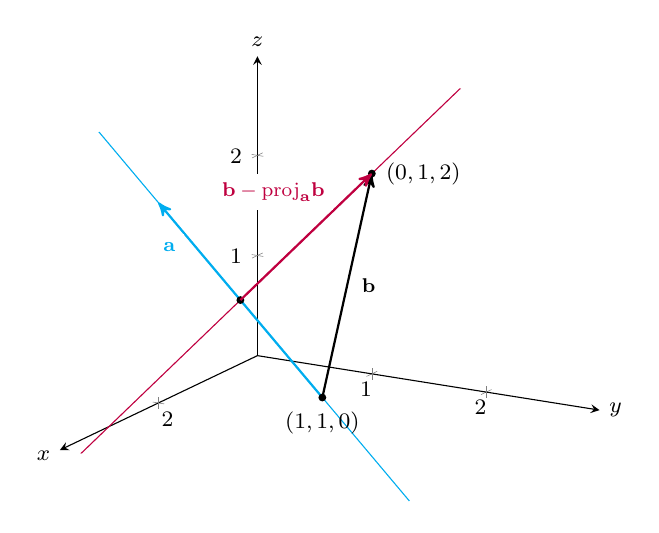
\begin{tikzpicture}[font=\footnotesize]
\pgfplotsset{compat=1.8}
\begin{axis}
[axis lines = center, view={120}{20},
axis background, xlabel = {$x$}, ylabel ={$y$}, zlabel ={$z$}, domain =-2:2, y domain =-2:2,
xmin =0,
xmax =3.99,
ymin =0,
ymax =2.99,
zmin =0, 
zmax =2.99,
samples =10, samples y =40, z buffer = auto, 
every axis x label/.style={
    at={(ticklabel* cs:1)},
    anchor= east, yshift =-2
},
every axis y label/.style={
    at={(ticklabel* cs:1)},
    anchor= west,
},
every axis z label/.style={
    at={(ticklabel* cs:1)},
    anchor= south
}]

\addplot3 [data cs=cart, cyan, domain=0:1, y domain = -1:2.3] ({2-y},{y},{2*(1-y)});

\addplot3 [thick, ->, >=stealth'] coordinates
{ (1,1,0) (0,1.0001,2) }node[right, fill=white, midway, pos=0.5, xshift=2, yshift=0, scale=0.9]{${\bf b} $};

\addplot3 [cyan, thick, <-, >=stealth'] coordinates
{ (2,0,2) (1,1,0) }node[below, fill=white, midway, pos=0.1, xshift=-2, yshift=-4, scale=0.9]{${\bf a}$};

\addplot3 [data cs=cart, purple, domain=0:1, y domain = -1:2.3] ({-3*(y-1)},{y},{2+2*(y-1)});

\node[label={0:{$(0,1,2)$}},circle,fill,inner sep=1pt] at (axis cs:0,1,2) {};
\node[label={-90:{$(1,1,0)$}},circle,fill,inner sep=1pt] at (axis cs:1,1,0) {};

\node[label={180:{${}$}},circle,fill,inner sep=1pt] at (axis cs:1.5,0.5,1) {};

\addplot3 [purple, thick, ->, >=stealth'] coordinates
{ (1.5,0.5,1) (0,1,2) }node[left, fill=white, midway, pos=0.7, xshift=0.6, yshift=7, scale=0.9]{${\bf b} - \hbox{proj}_{\bf a} {\bf b}$};

\end{axis}

\end{tikzpicture}
\end{document}